\headerbox{\bf\color{sufered} Experiments}
{name=experiments,column=2,row=0,span=3}
{
    \begin{minipage}[t]{0.5\textwidth}
        \textbf{\color{sufered}Synthetic Datasets for Training:} 
        \vspace{-0.2em}
        \begin{center}
            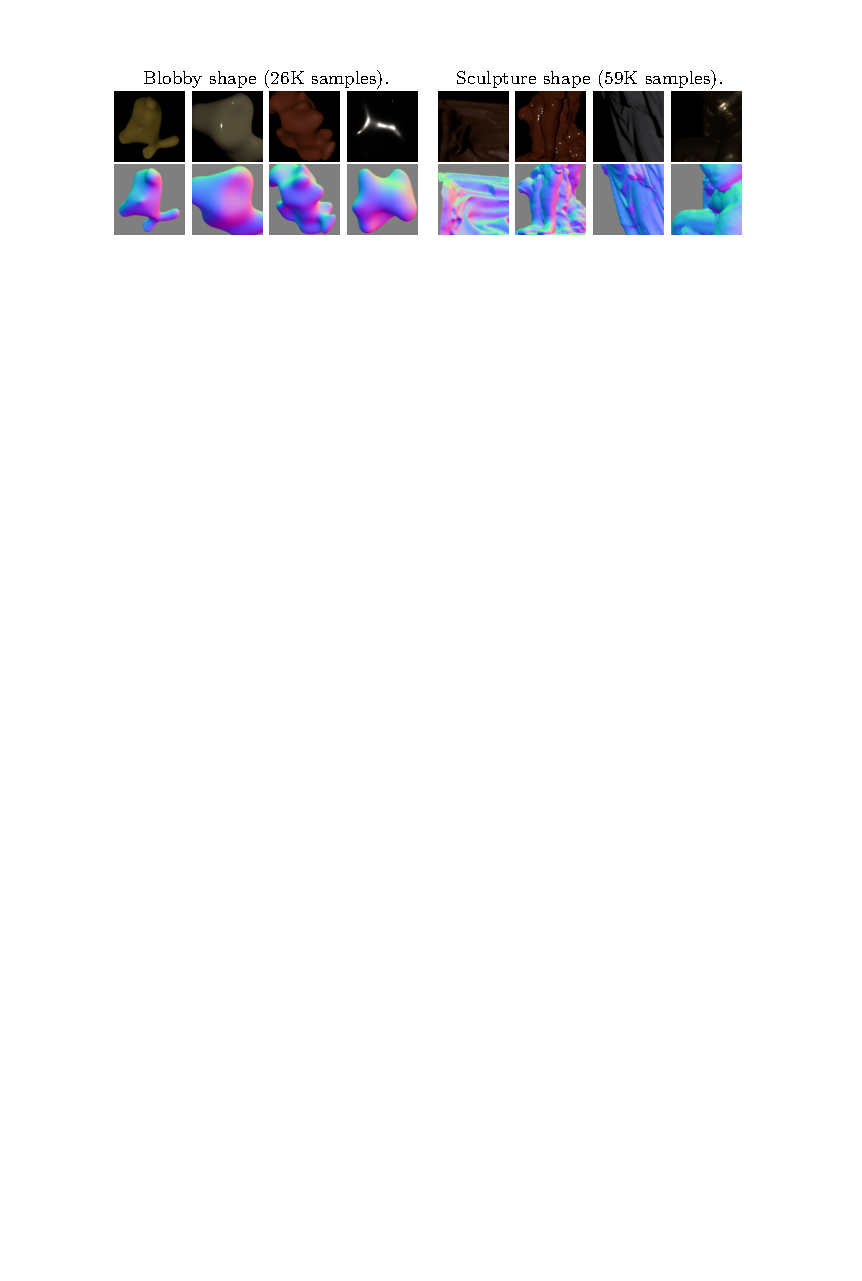
\includegraphics[width=\textwidth]{images/datasets.pdf}
        \end{center}
    \end{minipage}
    \begin{minipage}[t]{0.5\textwidth}
        \textbf{\color{sufered}Quantitative Results on DiLiGenT Main Dataset:} 
        \vspace{-0.2em}
        \begin{center}
            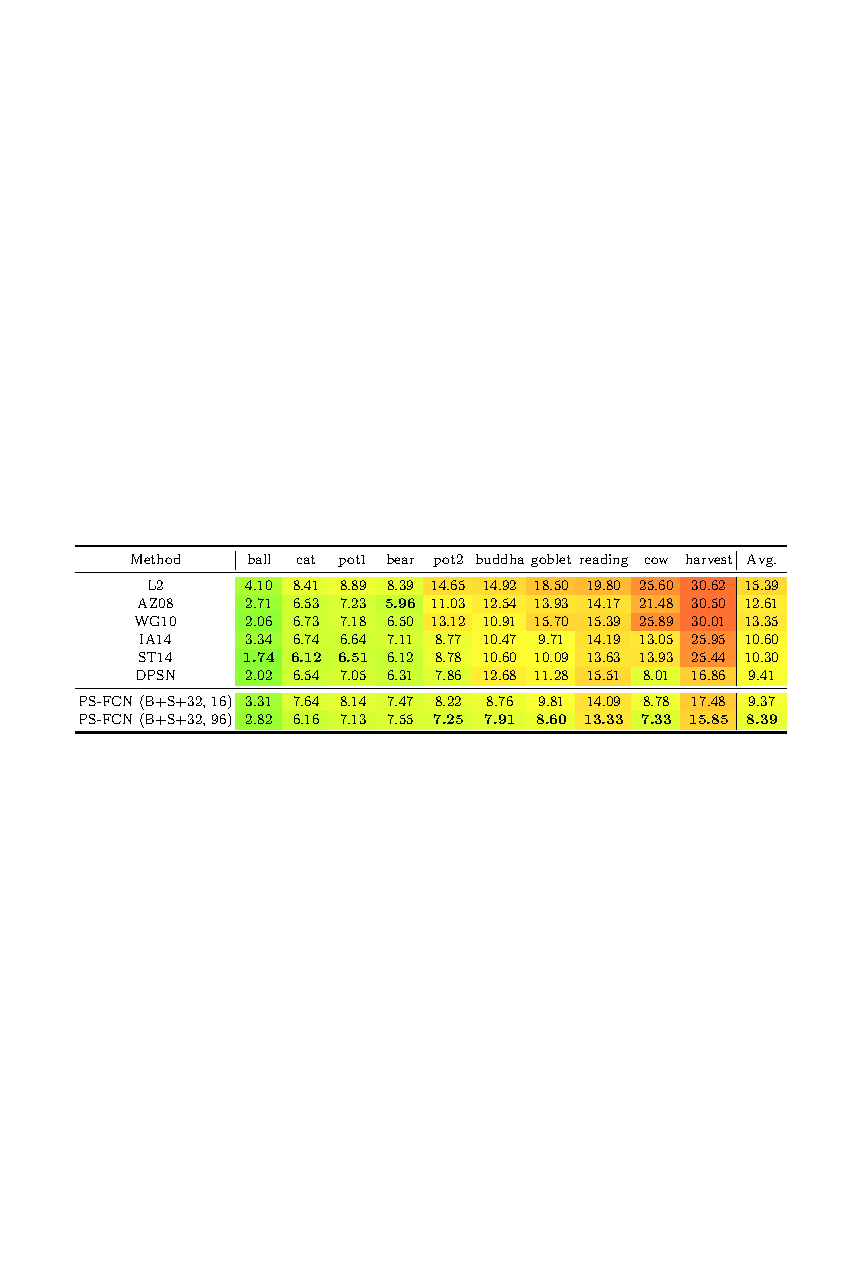
\includegraphics[width=0.98\textwidth]{images/res_quant_diligent_main}
        \end{center}
    \end{minipage}

    \vspace{0.5em}

    \begin{minipage}[t]{0.525\textwidth}
        \textbf{\color{sufered}Feature Visualization:}
        \vspace{-0.5em}
        \begin{center}
            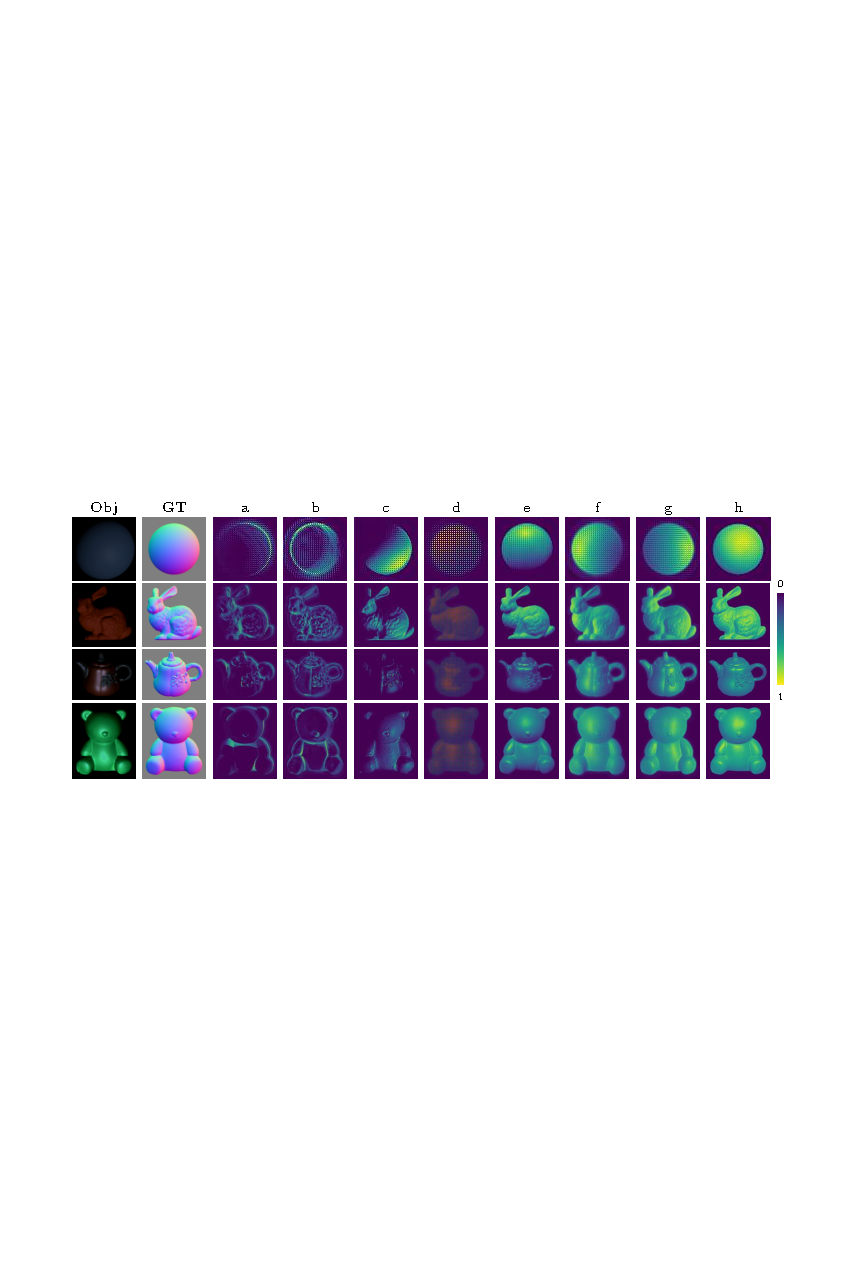
\includegraphics[width=\textwidth]{images/visualization}
        \end{center}
        \vspace{-0.9em}
        \begin{itemize}
            \item Different regions with similar normal directions are fired in different channels. Each channel can therefore be interpreted as the probability of the normal belonging to a certain direction.
        \end{itemize}
    \end{minipage}
    \hfill
    \begin{minipage}[t]{0.465\textwidth}
    \textbf{\color{sufered}Qualitative Results on DiLiGenT Main Dataset:} 
        \begin{center}
            \vspace{-0.5em}
            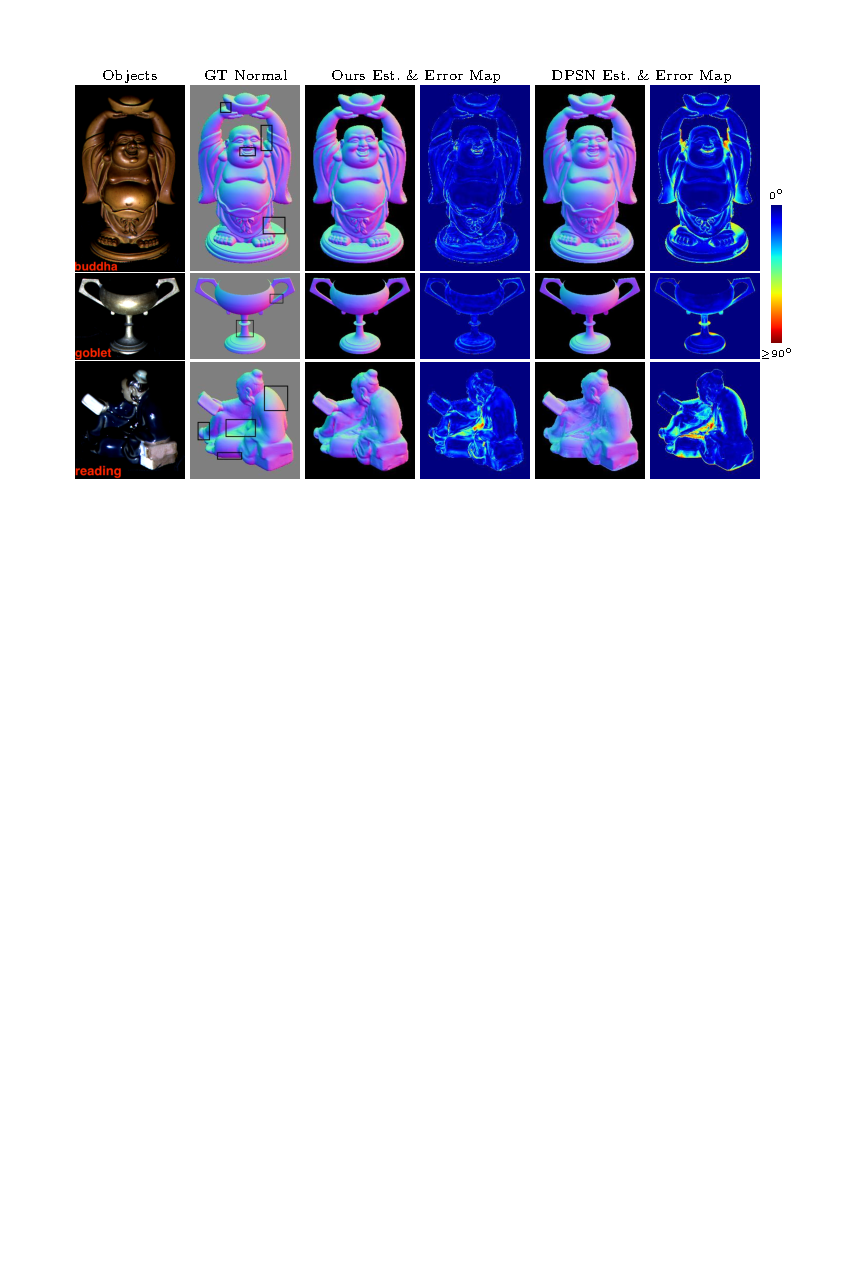
\includegraphics[width=\textwidth]{images/res_qual_diligent_main}
        \end{center}
    \end{minipage}

    \vspace{0.8em}
    \textbf{\color{sufered}Qualitative Results on the Gourd\&Apple Dataset and Light Stage Data Gallery:}
    \vspace{-0.8em}
    \begin{center}
        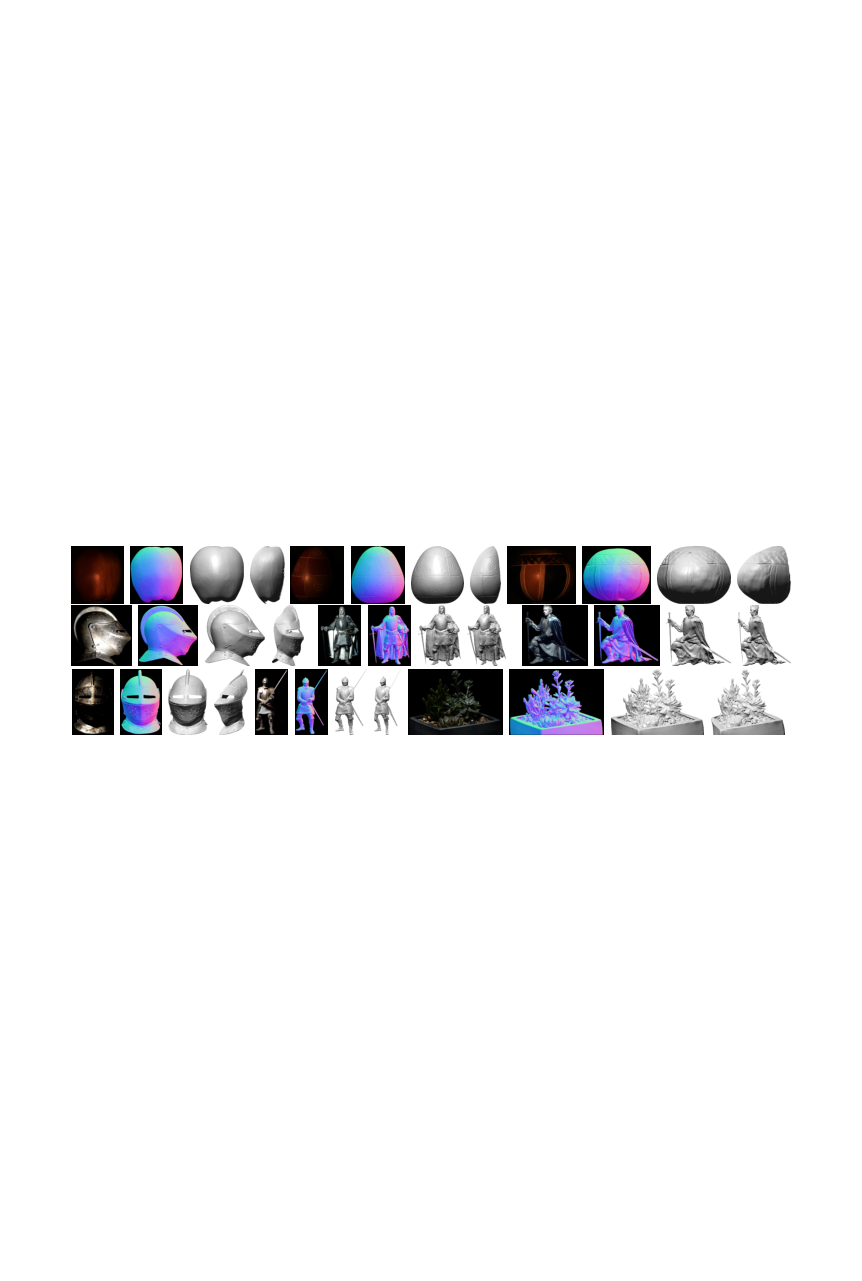
\includegraphics[width=1\textwidth]{images/gourd_stage}
    \end{center}

    \begin{minipage}[t]{0.6\textwidth}
        \textbf{\color{sufered}Quantitative Results on Spheres Rendered with 100 Different Materials:} 
        \vspace{-0.5em}
        \begin{center}
            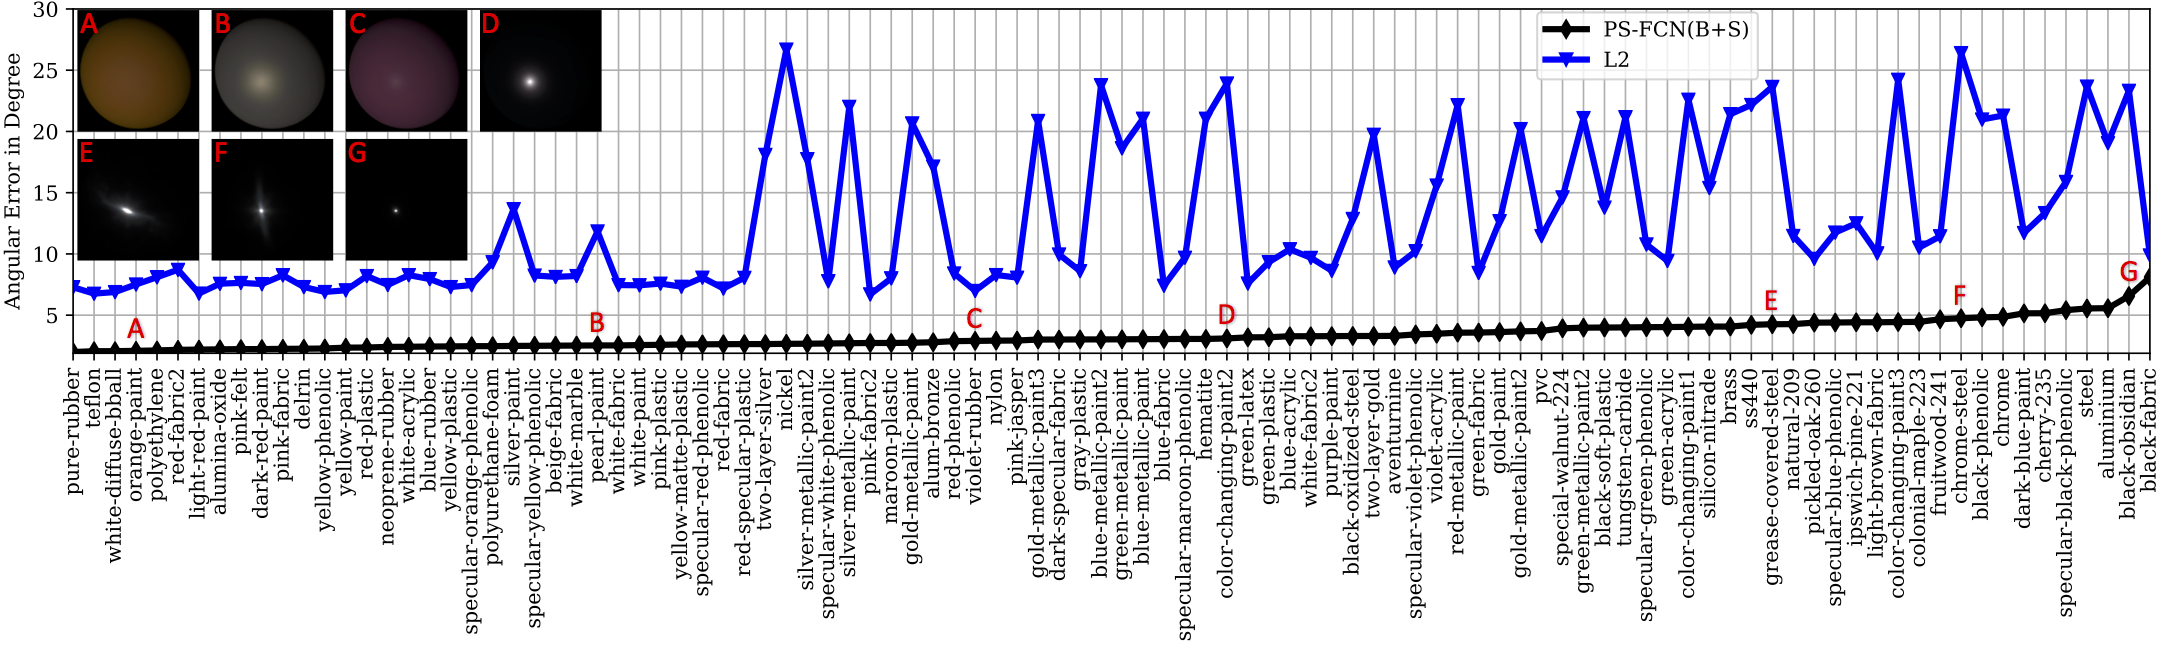
\includegraphics[width=\textwidth]{images/100brdf.png}
        \end{center}
    \end{minipage}
    \begin{minipage}[t]{0.4\textwidth}
        \textbf{\color{sufered}Quantitative Results of Uncalibrated PS-FCN on DiLiGenT Main Dataset:} 
        \vspace{-0.5em}
        \begin{center}
            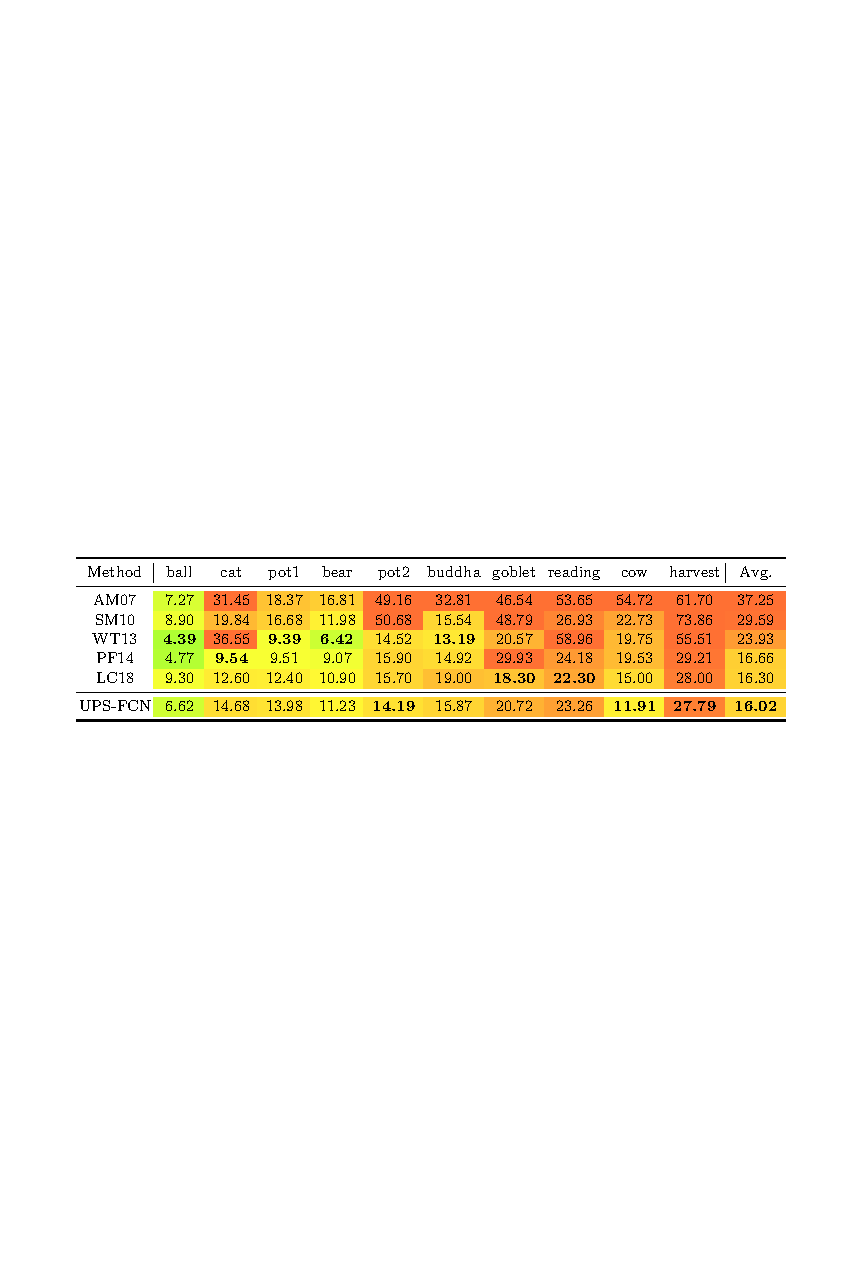
\includegraphics[width=\textwidth]{images/res_uncalibrated}
        \end{center}
        \vspace{-1.5em}

        \begin{center}
        \begin{minipage}{0.56\linewidth}
            \begin{center}
            \textbf{Project Webpage}: \\
            \vspace{0.5em}\textbf{Code} \& \textbf{Dataset} \& \textbf{Model}
            \end{center}
        \end{minipage}
        \begin{minipage}{0.24\linewidth}
            \begin{center}
                
\includegraphics[width=\linewidth]{images/PS-FCN_QRCode.png}
            \end{center}
        \end{minipage}
        \end{center}
    \end{minipage}
}